\section{Admin CRUD}
Para poder realizar el CRUD de los modelos en Django, se debe registrar los modelos en el archivo admin.py de cada aplicación. A continuación se muestra un ejemplo de cómo se registra el modelo Course en el archivo admin.py de la aplicación courses:

\begin{lstlisting}[language=Python]
from django.contrib import admin
from courses.models import Course
from courses.models import Content
from courses.models import Assignment
from users.models import Student
from users.models import Teacher
from groups.models import Group


# Register your models here.
admin.site.register(Course)
admin.site.register(Content)
admin.site.register(Assignment)
admin.site.register(Student)
admin.site.register(Teacher)
admin.site.register(Group)
\end{lstlisting}

Esta es una forma de registrar los modelos en el panel de administración de Django, para poder realizar el CRUD de los modelos.

Aqui se muestra el acceso por medio de la URL /admin, donde se puede ver los modelos registrados en el panel de administración de Django.

\begin{figure}[H]
  \centering
  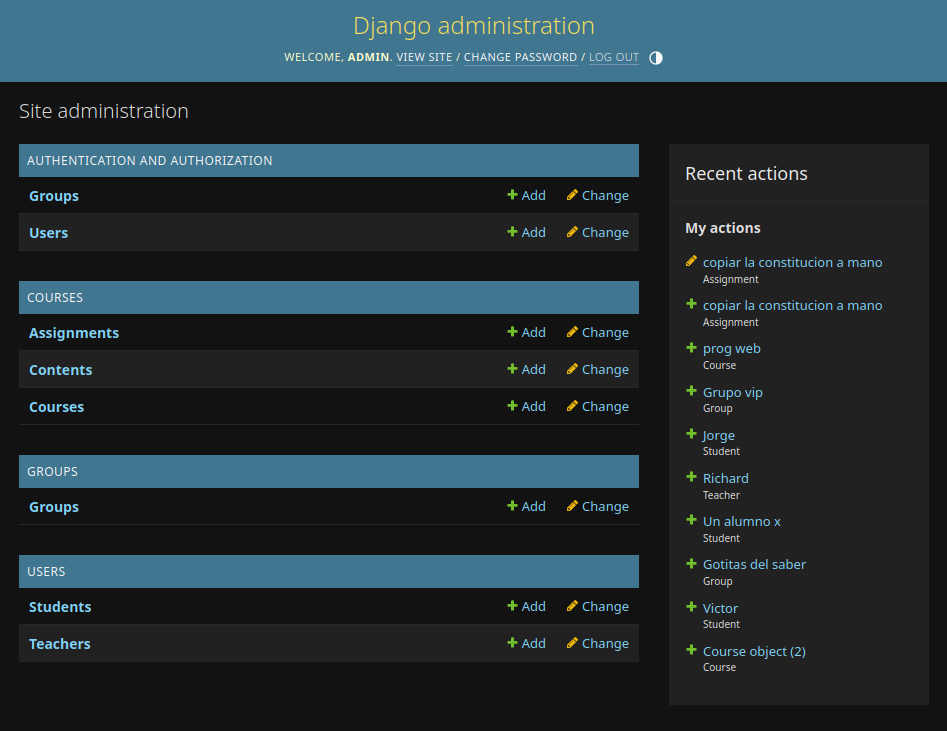
\includegraphics[width=0.8\textwidth]{img/admin.png}
  \caption{Panel de administración de Django}
\end{figure}

